\documentclass[solution,addpoints,12pt]{exam}
\usepackage{amsmath}
\usepackage{amsthm}
\usepackage{amssymb,graphicx}

\newtheorem{theorem}{Theorem}
\newtheorem{lemma}[theorem]{Lemma}

\newenvironment{Solution}{\begin{EnvFullwidth}\begin{solution}}{\end{solution}\end{EnvFullwidth}}

\printanswers
%\unframedsolutions
\pagestyle{headandfoot}

%%%%%%%%%%%%%%%%%%%%%%%%%%%%%%%%%%%%%%%%%%%%%%%%%%%%%%
%%%%%%%%%%%%%%%%%%% INSTRUCTIONS %%%%%%%%%%%%%%%%%%%%%
% * Fill in your name and roll number below

% * Answer in place (after each question)

% * Use \begin{solution} and \end{solution} to typeset
%   your answers.
%%%%%%%%%%%%%%%%%%%%%%%%%%%%%%%%%%%%%%%%%%%%%%%%%%%%%%
%%%%%%%%%%%%%%%%%%%%%%%%%%%%%%%%%%%%%%%%%%%%%%%%%%%%%%

% Fill in the details below
\def\studentName{\textbf{TODO: Name}}
\def\studentRoll{\textbf{TODO: Roll}}

\firstpageheader{CS 6841 - Mid-Semester}{}{\studentName, \studentRoll}
\firstpageheadrule

\newcommand{\brac}[1]{\left[ #1 \right]}
\newcommand{\curly}[1]{\left\{ #1 \right\}}
\newcommand{\paren}[1]{\left( #1 \right)}
\newcommand{\card}[1]{\left\lvert #1 \right\rvert}

\newcommand{\prob}{\operatorname{\mathbf{Pr}}}
\newcommand{\ex}{\operatorname{\mathbf{E}}}
\newcommand{\from}{\leftarrow}

\newcommand{\field}{\mathbb{F}}
\newcommand{\reals}{\mathbb{R}}
\renewcommand{\mod}{\operatorname{mod}}
\newcommand{\hashFamily}{\mathcal{H}}

\newcommand{\Yes}{\texttt{Yes}}
\newcommand{\No}{\texttt{No}}

\begin{document}

\begin{questions}

\question[25] \textbf{(Flows, Cuts, and Expander Graphs)}
You should recall the famous \emph{max-flow min-cut theorem} which ascertains the following beautiful theorem: given a undirected graph $G = (V,E)$ where each edge has unit capacity, and a source vertex $s$ and sink vertex $t$, consider the two quantities: Let $F_{\max}$ denote the maximum flow which $s$ can send to $t$ while respecting edge capacities; let $C_{\min}$ denote the minimum number of edges crossing any partition of the form $(S,V\setminus S)$ where $s \in S$ and $t \in V \setminus S$. Then $F_{\max} = C_{\min}$. In fact, one such proof of this theorem is by using LP duality. In this question, we will study the same from a more practical setting.

In this question, there are many source,destination requests of the form $(s_1, t_1)$, $(s_2, t_2)$, $\ldots, (s_k, t_k)$ where $s_1$ wants to send some flow to $t_1$, $s_2$ wants to send some flow to $t_2$, and so on. The goal is to maximize the total throughput, i.e., send some $\lambda_i$ flow from $s_i$ to $t_i$ such that $\sum_{i} \lambda_i$ is maximized. You may assume that all sources are sinks are distinct vertices (i.e., no $s_i$ is the same vertex as another $s_j$ or $t_j$).

We now state below, the Linear Program which captures this problem. The set $P_{(s_i,t_i)}$ is the set of all simple paths from $s_i$ to $t_i$, and every element $p \in P_{(s_i,t_i)}$ is a simple path from $s_i$ to $t_i$. Ignore the fact that there are exponentially many variables --- we are not trying to implement this in a computer, we are only using LPs to understand/prove some very fundamental mathematical properties about flows and cuts in this question. In fact, this exercise shows how to use algorithmic techniques like LPs and Duality to show deep mathematical properties.

\begin{alignat*}{2}
\max  & \sum_{i=1}^{k} \lambda_i \\
\text{s.t}  & \sum_{p \in P_{(s_i,t_i)}} f_p \geq \lambda_i & \qquad  \forall 1 \leq i \leq k  \\
  & \sum_{i} \sum_{p \in P_{(s_i,t_i)} \, {\rm s.t } \, e \in p} f_p  \leq 1 & \qquad \forall e \in E \\
  & f_p \geq 0 & \qquad \forall i, \forall p \in P_{(s_i,t_i)}
\end{alignat*}

\begin{parts}
\part[5] Let $F_{\max}$ then denote the maximum flow, i.e., optimum value of the above LP. Likewise, analogous to $C_{\min}$ defined above, we can define a similar cut value: consider partitioning the graph vertices into disjoint sets $S_1$, $S_2$, $\ldots, S_p$ for any $2 \leq p \leq n$. Call such a partition a \emph{separating partition} if for each $1 \leq i \leq k$, $s_i$ and $t_i$ are in different sets (i.e., all sources and sinks are separated). As an extreme example, the partition where each vertex is in its own set $\{v\}$ is one such separating partition with $t = n$. Now, let $C_{\min}$ denote the \emph{fewest number of edges cut} (which go between different sets) among all separating partitions. Show that $F_{\max} \leq C_{\min}$.

  \begin{solution}
  \begin{proof}
  $1 + 1 = 2$.
  \end{proof}
  \end{solution}


\part[10] Consider the following instance in Figure~\ref{figure1}, and show that $F_{\max}$ can be strictly smaller than $C_{\min}$. This shows that having more than one source or sink makes the max flow-min cut theorem false!

\begin{figure}
  \centering
  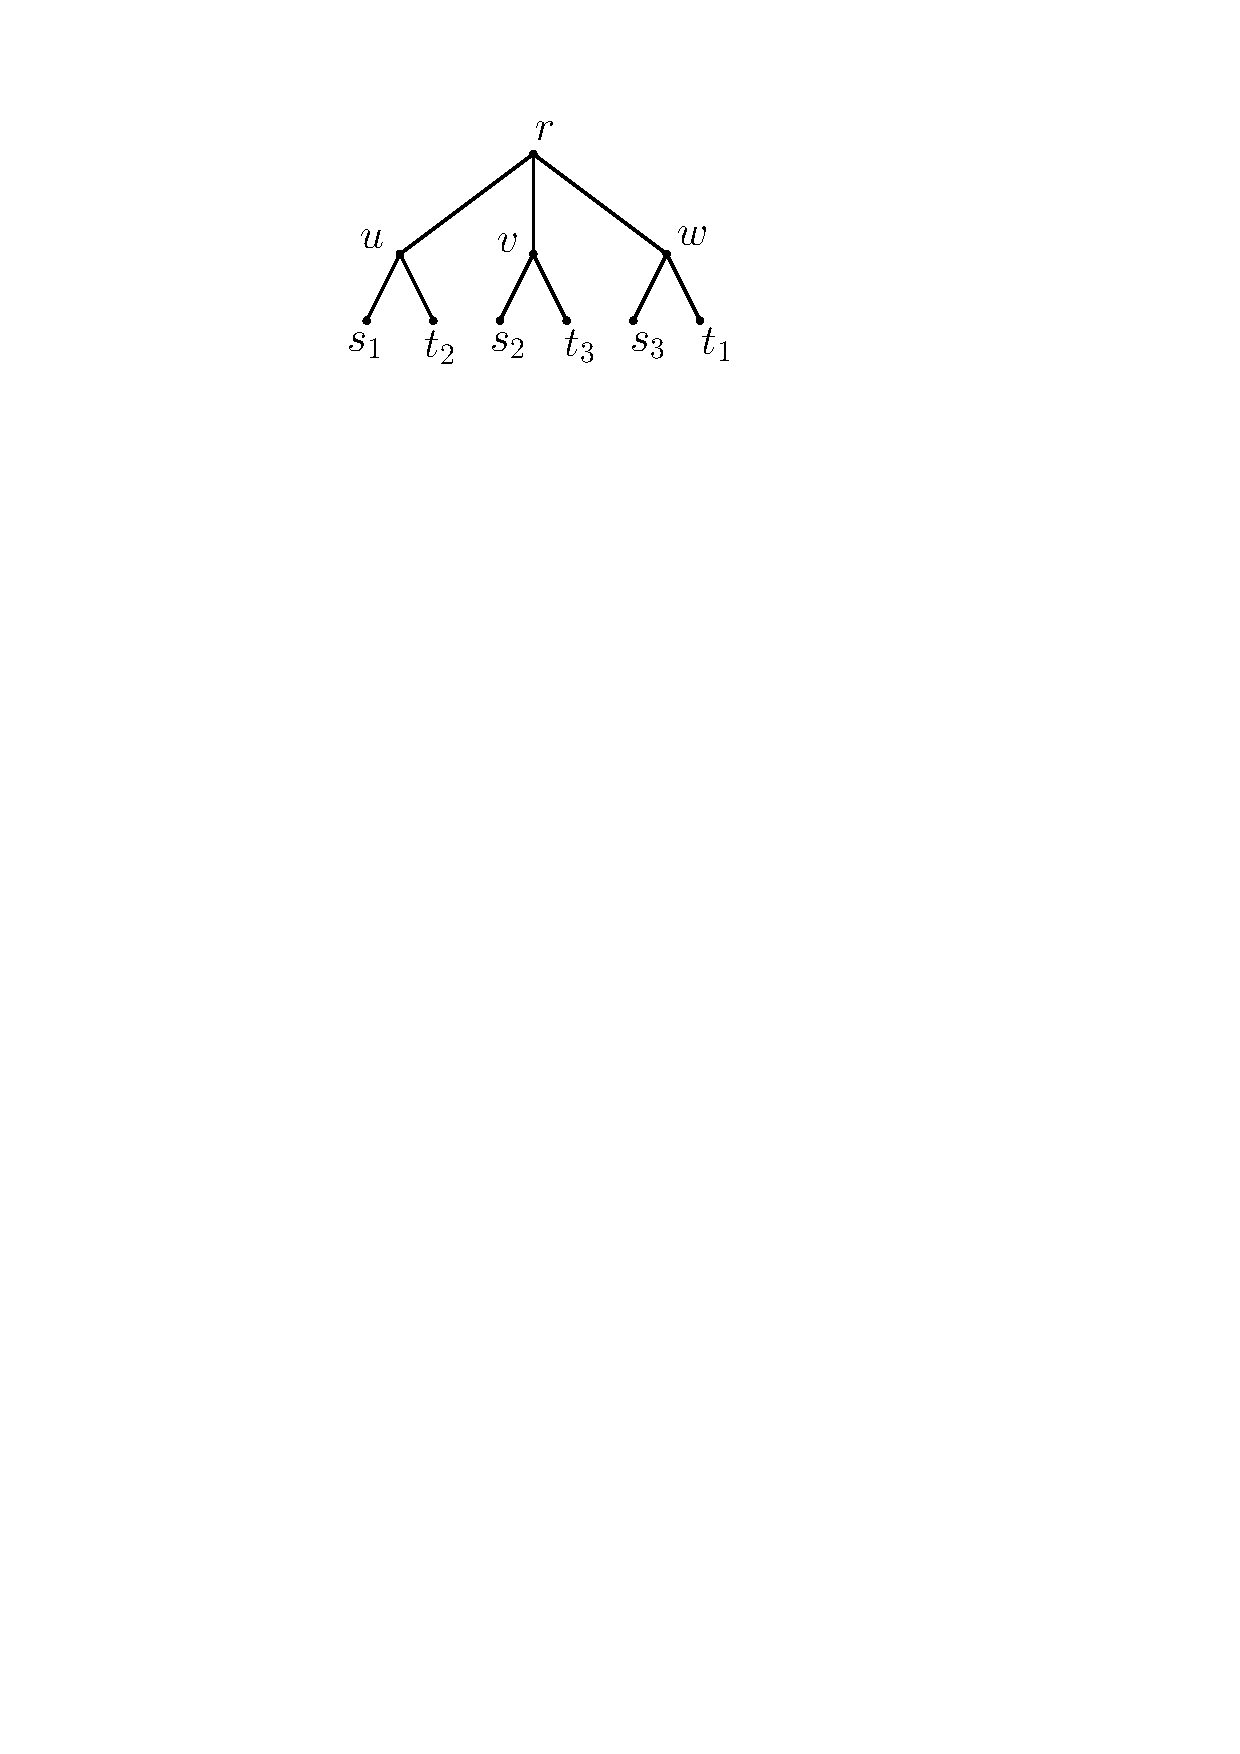
\includegraphics[scale=0.8]{gap-eg.pdf}
  \caption{Figure for Gap Example}
  \label{figure1}
\end{figure}

  \begin{solution}
  \begin{proof}
  $1 + 1 = 2$.
  \end{proof}
  \end{solution}


\part[10] Write the dual of the LP above, and say why it is the \emph{LP relaxation} of the problem of finding the minimum cut defined above in part (a).

  \begin{solution}
  \begin{proof}
  $1 + 1 = 2$.
  \end{proof}
  \end{solution}



\end{parts}


\question[20]  \textbf{(Guessing the Last Heads)}
You are given a sequence of $n$ coin numbered $1$ through $n$, and values $p_1$, $p_2$, $\ldots, p_n$ between $[0,1]$ which denote the probability that the $i^{th}$ coin comes up heads; these are all independent of each other. Then I toss these coins one by one, starting with the first coin. If you see a head, then your goal is to predict if that will be the last head in the sequence, i.e., there will be no more heads. You have only one chance to make such a prediction, and you win if you are correct, that is, I finish tossing all remaining coins and find no further head. Your task is to devise the \emph{optimal strategy} to maximize the probability of winning. Recall you know all the $p_i$ values, so use this in wisely deciding when to make the prediction. Also recall you have only one chance of making a prediction, that is, say you have seen the $10^{th}$ coin and it is a head, and you decide to predict that it is the last head. Then you win only if coins $11$ through $n$ all turn up tails.

Most of modern day resource allocation algorithms have such stochastic information handy, and need to make online decisions as above. Understanding this framework will prepare you to tackle these very real challenges system-designers face. The key lies in correctly modeling the systems challenges in a clean algorithmic manner. Once you do that, techniques like what you will devise for this question will immensely help you.

({\bf Hint:} use Dynamic programming, using the value $V_i$ which denotes the optimal success probability of predicting correctly when only coins $i$ through $n$ are at play, i.e., you have seen and skipped the first $i-1$ coins and can only make predictions on $i$ through $n$. For example, $V_n$ is simply $p_n$, as you can predict with certainty if you see a head, which happens with probability $p_n$.)

  \begin{solution}
  \begin{proof}
  $1 + 1 = 2$.
  \end{proof}
  \end{solution}


\question[15] \textbf{(Quickly Testing Matrix Product)}
You are given three $n \times n$ matrices $A, B, C$, and want to check if $C = AB$ reasonably quickly.

\begin{parts}
\part[3] What's the naive way to solve this problem? What is the running time complexity?
  \begin{solution}
  \begin{proof}
  $1 + 1 = 2$.
  \end{proof}
  \end{solution}

\part[12] Now let's devise a randomized algorithm which is significantly faster that your naive solution. Such ideas are the key takeaways from this course, demonstrating the power of cleverly using randomness. Indeed, pick a random binary vector $f \in \{0,1\}^n$ where each coordinate is $0$ or $1$ with probability $\frac12$ independently. Show that $AB f = Cf$ always holds if $AB = C$, and holds with probability at most $1/2$ if $AB \neq C$.


  \begin{solution}
  \begin{proof}
  $1 + 1 = 2$.
  \end{proof}
  \end{solution}


\part[10] Even if you couldn't prove part (b), assume it is true. How do you boost the failure probability to $\epsilon$. What is the overall running time of this algorithm which fails with at most $\epsilon$ probability. Be clever in testing whether $AB f = Cf$ quickly.


  \begin{solution}
  \begin{proof}
  $1 + 1 = 2$.
  \end{proof}
  \end{solution}


\end{parts}


\end{questions}
\end{document} 